\documentclass[12pt]{article}
\usepackage[a4paper]{geometry}
% Let's add some line spacing to make it readable
\renewcommand{\baselinestretch}{1.15}

\usepackage{graphicx}
\graphicspath{{figures/}}
\geometry{verbose,tmargin=2.5cm,bmargin=2.5cm,lmargin=2.5cm,rmargin=2.5cm,columnsep=1.5cm}
\usepackage{amssymb}
\usepackage{amsmath}
\usepackage{tabu}
\usepackage{booktabs}


\DeclareMathOperator*{\argmin}{arg\,min}

\title{\Large Vitamin A Supplements and Child Mortality:\\ Resolving A Controversy In Meta-Analysis\\
%\Large \color{red} EMBARGOED COPY. \\
%PLEASE DO NOT CIRCULATE. 
}
\author{Rachael Meager\footnote{University of New South Wales. Contact: R.Meager@lse.ac.uk.}, Witold Więcek\footnote{Development Innovation Lab, University of Chicago}\;\thanks{We thank Abhijit Banerjee, Esther Duflo, Anna Mikusheva, Victor Chernozhukov and Alfred Sommer for helpful discussions and suggestions. All remaining mistakes are our own. This is a working paper. Please send critiques and corrections via email.  }}


\begin{document}
\maketitle

\begin{abstract}
Vitamin A supplementation is considered one of the most effective interventions to reduce child mortality in developing nations. However, its estimated effect varies substantially across studies, making the results of meta-analyses in this literature highly sensitive to methodological choices. 

We compare the theoretical properties and empirical performance of classical fixed-effects and  random-effects meta-analysis models on simulated bodies of evidence. We consider Bayesian implementation using a hierarchical model. We find that using random effects either matches or substantially outperforms the fixed effects method in terms of mean squared error and is robust to misspecification of the likelihood. 

Applied to a set of 18 studies, a Bayesian model estimates that vitamin A supplementation reduces mortality risk by 25\% (95\% interval 40\% to 11\%), compared to 12\% under the fixed-effects model (95\% interval 7\% to 17\%). 
The model suggests that the underlying heterogeneity across studies is large (66\% of the cross-study variation attributable to genuine differences in treatment effects), but this is not precisely estimated (95\% interval 26\% to 91\%).
Fixed effects thus underestimate both the reduction in mortality and the uncertainty surrounding the general effect of supplementation. 

\end{abstract}

\section{Introduction}
% vitamin A is a big deal - Sommer discovery and subsequent literature 
Public health researchers and international aid organisations consider vitamin A supplementation one of the most important and cost-effective interventions to reduce child mortality (Imdad et al 2022, Bill and Melinda Gates Foundation 2011). UNICEF refers to vitamin A programming as a ``prerequisite'' for achieving Millenium Development Goal 4, the goal of child survival, particularly in countries with high vitamin A deficiency rates (UNICEF, 2007).  The potential of large-scale vitamin A supplementation to effectively reduce child mortality was first established in Sommer et al (1986) using a randomized controlled trial in Sumatra, Indonesia; the program reduced child mortality by 34\% of base risk. The literature that followed displayed substantial variation in results across different contexts, but often confirmed or strengthened the initial finding (see for example Vijayaraghavan et al 1990, Rahmathullah et al 1990, Herrera et al 1992, Arthur et al 1992, VAST 1993). 

%WW: does this need a short paragraph explaining FE vs RE upfront? DEVTA trial meta-analysis may not make sense otherwise
%JM: I don't think that's necessary, but what do I know

% - biological underpinnings 
The biological mechanism by which vitamin A affects mortality is relatively well understood: retinoic acid has a specific role in visual system function and in the immune system where it improves T and B cell gut-homing capacity and enhances T cell proliferation (Mora et al, 2008 and Iwata et al 2004). This explains why vitamin A deficiency is often associated with greater mortality risk in longitudinal data (Sommer et al, 1983). While the effect of supplementation in the absence of vitamin A deficiency is unclear, this deficiency is prevalent in so many developing countries that the World Health Organisation recommends general supplementation (WHO, 2016). 
Recent meta-analyses have concluded that the average risk ratio of supplementation is 0.76 and thus recommend universal supplementation (Mayo-Wilson et al 2011, Imdad et al 2022). 

% Then DEVTA is happen, by far the most precise, but perhaps a very different context 
However, some recent results from the largest ever randomised controlled trial (RCT) of vitamin A supplementation threaten to overturn this consensus (Awasthi et al, 2013). The study, performed in India, reported only a small and statistically insignificant reduction in child mortality. This was not the first time a study had found no effect of vitamin A, and one previous study even found a slight and insignificant increase in mortality (Herrera et al, 1996). But Awasthi et al (2013), often called the ``DEVTA trial'', studied millions of subjects and produced the most precise estimate of the risk ratio ever recorded. However, despite this impressive precision, the DEVTA trial was unusual in many ways: in particular, it had a different delivery mechanism and a lower rate of compliance relative to other studies (Awasthi et al 2013, Sommer et al 2013). As a result, some researchers remain unconvinced that the DEVTA trial should meaningfully overturn or alter the conclusions of the previous three decades of research on Vitamin A (Sommer et al, 2013, and Garner et al, 2013).

% so how do we interpret this literature? It turns out to be sensitive to how we aggregate the results
Faced with severe disagreements in the scientific community about the implications of a body of research, the methodological question of how to aggregate and interpret the evidence from seemingly-contradictory studies becomes crucially important. This question has material consequences for science and policy, because the conclusions of evidence aggregation exercises are often sensitive to the statistical methodologies chosen in these contexts. Both Imdad et al (2011) and Awasthi et al (2013) fit a fixed-effects meta-analysis model and found a risk ratio of 0.89, a difference of more than ten percentage points from the meta-analyses using random-effects (Mayo-Wilson et al 2011, Imdad et al 2022).\footnote{In the economics literature, terms "constant effects" and "random coefficients" are used for fixed and random effects respectively.} Sommer et al (2013) note the heterogeneity in the results and suggest that a random effects aggregation model would produce more reliable results. Awasthi et al (2013) claim that random effects meta-analytic techniques overweight small studies, and "conceal the reliability" of large studies such as DEVTA; Sommer et al (2013) argue that fixed effects techniques underweight small studies and overweight large trials.\footnote{Imdad et al. discuss the results as follows: ``We acknowledge that the addition of DEVTA trial 2013 results decreased the overall effect size for this outcome compared to previous analysis for this review. However, we consider that vitamin A has robust effects on mortality as the direction of effect is in favour of intervention in most of the studies and summary estimate remains statistically significant irrespective of the use of random‐ or fixed‐effect models''} 

% this paper asks theoretically and empirically which method should be used in this literature 
In this paper, we investigate which method should be used to aggregate the evidence in the vitamin A literature, and apply that method to perform a new meta-analysis. We review the theoretical properties of fixed and random effects estimators and investigate their empirical performance on simulated literatures. 
%WW: I don't understand the next point: the paper later states that our results don't change if (some sort of) MLE estimation is used to fit RE models, but we list "used non-Bayesian methods" (and their problems) as a motivation for this work
%WW: Rachael says let's add more explanation qualitatively when discussing the RE vs BHM split in Methods
Earlier work by Hedges and Vevea (1998), Overton (1998), and Field (2001) reported simulation studies assuming that the functional form of either the fixed-effects (FE) model or the random-effects (RE) model was exactly correct, used non-Bayesian RE methods (which are known to have problems, including underestimating heterogeneity: see Cornell et al 2014, Brockwell and Gordon 2001), and scored performance by type 1 error rate. By contrast, we examine performance on a wider range of data-generating processes for which neither meta-analytic model is exactly correct, including distributions with fat tails and multi-modal mixture distributions. To assess performance, we conduct a Monte Carlo simulation and compare the mean squared error (MSE) of both procedures in estimating the average treatment effect. This approach is chosen over evaluating hypothesis test error rates. We do this because research communities are increasingly interested in getting an estimate as close as possible to the true effect size, not simply testing for the existence of a non-zero effect (Wasserstein and Lazar 2016). We then fit both FE and RE models using data from the most recent meta-analysis by Imdad et al. (2022) and conduct a formal comparison of these two models.



\section{Methodologies for Meta-Analysis}

\subsection{Fixed Effects}

% if we're confident the effects are the same, inv-var is optimal
The canonical fixed-effects meta-analysis model uses an inverse-variance weighted average of the studies' estimated effects to produce an estimate of a general or typical treatment effect (Higgins and Green, 2011, 9.4.3). For a set of $K$ studies with estimated treatment effects and reported standard errors  $\{\hat{\tau}_k, se_k\}_{k=1}^K$, the FE estimator is

\begin{equation}
\label{fe_tau}
\begin{aligned}
\hat{\tau}_{FE} = \sum_{k=1}^K \hat{\tau}_k \frac{  (se^2_k)^{-1}   }{  \sum_{k=1}^K  (se^2_k)^{-1}  } \; \; .
\end{aligned}
\end{equation}
The standard error of this estimate is calculated as follows:

\begin{equation}
\label{fe_se}
\begin{aligned}
\hat{se}_{FE} = \sqrt{ \frac{ 1  }{  \sum_{k=1}^K  (se^2_k)^{-1}  }} \; \; .
\end{aligned}
\end{equation}

If the studies are estimating the same underlying treatment effect $\tau$, and each study's estimated effect $\hat{\tau}_k$ is asymptotically  normally distributed, then this method is optimal in the class of estimators produced by linear combinations of the $\{\hat{\tau}_k\}_{k=1}^K$. This result is proved in Hedges and Vevea (1998) but had been established informally in the statistics literature years prior. We review it here: formally, assume that the point estimators are consistent and that each study has enough data and the empirical distributions have enough regularity such that, for all $k$, $\hat{\tau}_k \sim \mathcal{N}(\tau, se^2_{k})$.\footnote{An assumption of this sort is typically made during the calculation of most standard parametric confidence intervals and p-values in the medical and social science literature.}

Now consider the class of estimators for which $\hat{\tau} = \sum_{k=1}^{K} w_k \hat{\tau}_k$ for 
for some positive weights, $\sum \{w_k\}_{k=1}^K =1$.
The sampling distribution of any such estimator will be

\begin{equation}
\begin{aligned}
\hat{\tau} \sim \mathcal{N}(\tau, \sum_{k=1}^{K} w_k^2 se^2_{k}) .
\end{aligned}
\end{equation}

Since all such estimators are consistent by construction, we seek estimator with the minimal mean squared error (MSE). Taking a first order condition with respect to the weights shows that

\begin{equation}\label{fe}
\begin{aligned}
\left\{ \frac{(se^2_k)^{-1}}{\sum_{k=1}^K(se^2_k)^{-1}} \right\}_{k=1}^K = \; \argmin_{ \{w_k\}_{k=1}^K  } \sum_{k=1}^{K} w_k^2 se^2_{k}.
\end{aligned}
\end{equation}

This result demonstrates the efficiency of the FE estimator in this class. Notice that the standard errors were ancillary statistics for $\tau$, yet are necessary to construct the efficient estimator. 

The FE model can be implemented using either a frequentist or a Bayesian approach. While the former is typically used, the Bayesian framework allows for direct comparison between fixed- and random-effects models, which we will discuss below. 



\subsection{Random Effects Methods}

%WW: this is unclear; I'd say: consider data generated by a process such that tau_k ~ Normal(tau, ...)
%WW: otherwise this assumption of normality just comes out of nowhere
%JM: I think this is sufficiently clear

If each $\hat{\tau}_k$ estimates a different $\tau_k$ rather than one common $\tau$, the FE estimator can be easily shown to diverge from the minimum-variance consistent estimator. To see this, consider a hypothetical case in which the $\{\hat{\tau}_k\}_{k=1}^K$ are estimates of $K$ distinct parameters according to the following hierarchical likelihood:

\begin{equation}\label{rubin}
\begin{aligned}
\hat{\tau}_k &\sim \mathcal{N}(\tau_k, se^2_{k}) \; \; \forall \;k\\
\tau_k &\sim \mathcal{N}(\tau, \sigma^2_{\tau}) \; \; \forall\; k.
\end{aligned}
\end{equation}

In this model, each $\hat{\tau}_k$ actually measures a $k$-specific underlying effect $\tau_k$, but these are centered around a common $\tau$ component. As before, we seek the minimum variance estimator of this $\tau$ given the estimates $\{\hat{\tau}_k, se_k\}_{k=1}^K$, in the class of estimators taking the form  $\hat{\tau} = \sum_{k=1}^{K} w_k \hat{\tau}_k$ for some positive weights, $\sum \{w_k\}_{k=1}^K =1$. 

By law of total variation and the properties of sum of normal distributions,

\begin{equation}
\begin{aligned}
\hat{\tau} \sim \mathcal{N}(\tau, \sum_{k=1}^{K} w_k^2( se^2_{k} + \sigma^2_{\tau})).
\end{aligned}
\end{equation}

%WW: Rachael to check my language
%JM: language looks good to me, but I may lack technical know-how
Since the estimator is consistent, the combination of weights that minimises MSE will lead to an efficient estimator. By the same argument that produced the optimal weights in the FE model, 

 \begin{equation}\label{efficient}
\begin{aligned}
\left\{ \frac{(se^2_k+ \sigma^2_{\tau})^{-1}}{\sum_{k=1}^K(se^2_k+ \sigma^2_{\tau})^{-1}} \right\}_{k=1}^K = \; \argmin_{ \{w_k\}_{k=1}^K  } \sum_{k=1}^{K} w_k^2 (se^2_{k}+ \sigma^2_{\tau}).
\end{aligned}
\end{equation}

Using these weights implements a random effects (RE) estimation method. When $\sigma^2_{\tau} \neq 0$, the FE estimator diverges from this estimator and has higher variance: the FE method is thus inefficient in this case. This is why the FE method is sometimes referred to as a ``full pooling'' method: it is only optimal when the data from all $K$ samples or studies estimates exactly the same effect. 

%The more heterogeneous the study settings, the less likely this is to be true, all else equal. 
When the true $\sigma^2_{\tau}$ is very large, the FE estimate may be very misleading. 
%WW: I remove this strong claim on the next line, since it may need some sort of proof:
%When treatment effects are heterogeneous across studies is statistically inefficient to let any single estimate strongly affect the estimated general effect, since each study still represents only 1 data point from the underlying distribution of treatment effects. 
The RE estimator accounts for underlying heterogeneity and thus tempers the influence that any single study can have on the estimate of $\tau$.

The RE estimator in \eqref{efficient} is optimal if $\sigma^2_{\tau}$ is known and if the effects are independently, identically, and normally distributed around their common mean. 
In practice, even if this functional form is correctly specified, $\sigma^2_{\tau}$ is not known and must be estimated. In fact this is the model described in Rubin (1981), which can be estimated via Bayesian inference or via Maximum Likelihood (which is often called ``Empirical Bayes'' in this case). For relatively simple models, such as \eqref{rubin}, the performance, computational complexity, and running time are similar for the two methods. 

In more complicated models, the ML estimation quickly becomes a challenging multivariate optimisation problem that requires inversion of large matrices to calculate standard errors. In these more complex cases, the ``Empirical Bayes'' MLE is performed using a 2-step procedure that does not accurately quantify the uncertainty in the unknowns. In general, frequentist random-effects meta-analytic estimators such as MLE are known to underestimate heterogeneity. In some cases, these estimators "snap to boundary" (i.e. estimate the heterogeneity parameter $\tau$ as zero) even when heterogeneity is present, but highly uncertain.\footnote{This occurs particularly often when the number of studies in a meta-analysis is low.}
%JM: is "snap to boundary" (above) a technical term?

\subsubsection*{Bayesian hierarchical model}

Our preferred alternative is to conduct inference on model \eqref{rubin} using a Bayesian hierarchical model (BHM). 

As with all Bayesian models, using this type of inference improves model checking and allows for generating posterior predictive quantities.\footnote{BHMs also avoid the boundary estimate problem faced by frequentist estimators, and can improve overall inference on heterogeneity by introducing informative or mildly informative priors (Chung et al, 2012). These priors can be derived from other meta-analyses in similar domains of study (Turner et al, 2015).} We use diffuse priors which ensure proper posterior influence. In the case of this meta-analysis, we find that our Bayesian meta-analytic defaults happen to agree with the frequentist REML estimator.
%We use diffuse priors which ensures proper posterior inference while (typically) leading to results extremely close to MLE.\footnote{We have verified that the MLE produces virtually identical results in the simple applications and simulations provided in this paper.} 
%JM: I don't think the above commented-out line should be included - seems confusing as BHM is supposed to be better than MLE but we're benchmarking it against MLE?

In this paper we estimate BHM using Hamiltonian Monte Carlo with a No-U-Turn-Sampler using Stan software.\footnote{Quality of approximation of the posterior distribution by the Monte Carlo methods depends not only on algorithm but also parameters such as the number of iterations (samples from the posterior). While in some cases this requires careful specification and troubleshooting, for meta-analysis models obtaining good convergence is easy to achieve. In this paper we use the standard Stan settings and check convergence via the $\hat{R}$ statistic proposed by Gelman and Rubin (1992).} This Bayesian approach to meta-analysis is implemented in an accessible way in the R package \textit{baggr}, which in addition to model \eqref{rubin} also includes other commonly used meta-analysis models (Więcek and Meager, 2022). The package also includes fitting of FE models, calculation of pooling statistics, and model selection through cross-validation, which we describe below.

\subsubsection*{Pooling metrics}

To formally quantify the heterogeneity in BHM we can compute the conventional pooling factor, as specified in Gelman et al (2006):

\begin{equation}
\omega(\tau_k) = \frac{\hat{se}^2_k }{\hat{se}^2_k + \hat{\sigma}_{\tau}^2 }
\end{equation}

When values of the pooling factor are close to 1, sampling variation in studies is much larger than cross-site heterogeneity. When pooling is low, cross-site heterogeneity dominates. This factor is the formal complement of the often-used $I^2$ metric (i.e. $I^2 = 1- \omega(\tau_k)$), reviewed favourably by Higgins and Thompson (2002), and provides the same information. 


\subsubsection*{Posterior predictive distributions}

%WW: Rachael to review this and edit
%JM: have edited the language but Rachael may still need to review the information content
The Bayesian approach to meta-analysis also allows for a straightforward calculation of the effect's posterior predictive distribution (p.p.d.). Generically, the p.p.d. tells the researcher what values the unobserved data could assume, conditional on observed data. In the case of meta-analyses, where we are interested in true treatment effects, this refers to a prediction of the effect in ``one additional study'', $\tau'$, and therefore the generalizability of the intervention. Under the FE model, the p.p.d. is trivially equal to the distribution of the mean treatment effect (since they are shared by each study). In other words, all of uncertainty in the p.p.d. is uncertainty in the estimate of the common effect. Under the RE model, variance is a sum of this uncertainty and heterogeneity ($\sigma_\tau^2$). 

\subsubsection*{Cross validation approach to model selection}

Using p.p.d's calculated under Bayesian implementation of FE and RE models offers researchers a possibility to compare the two models. We follow Gelman et al. (2014) in implementing leave-one-out cross-validation, a method of estimating model's out-of-sample performance. This is done by excluding one study at the time, refitting the model to remaining studies, and calculating predictive performance in terms of expected log predictive density (elpd).

\subsubsection*{Difficulty in choosing between RE and FE models}
%WW: maybe this needs shortening? breaking into 2 paras?
%JM: done, split into 2 paras
Even a researcher who is confident of heterogeneous effects cannot be certain of the distribution around the common effect $\tau$. The possibility of model error in the specification of the hierarchical model introduces some concern about the actual efficiency of any chosen RE estimator.\footnote{However, the RE estimator does have an important additional feature: 
%WW: I think this footnote is hard to follow. Is shrinkage a term familiar to readers? uniform domination? James-Stein estimator?
%JM: these terms aren't familiar to me (but I asked ChatGPT :))
it performs shrinkage which generates estimates of  $\{{\tau}_k\}_{k=1}^K$ that uniformly dominate $\{\hat{\tau}_k\}_{k=1}^K$ when $K \geq 3$ in terms of total mean-squared error even in the extreme case when the studies are statistically independent; this is proved in James and Stein (1961).} This problem does not imply that we should use the FE model instead, since if the underlying effects are heterogeneous then the FE estimator is also inefficient. Nor can we rely on popular tests of homogeneity in effects, as they typically have insufficient power to detect heterogeneity (Field, 2001). 

In practice, particularly for experiments performed in the field across different countries, researchers are often unwilling to rule out heterogeneity completely yet unhappy to draw inferences that are based on a potentially misleading specification of that heterogeneity. The relevant question then is which of the two meta-analytic approaches is likely to perform better in the presence of heterogeneity under a variety of conditions, and in particular, when the RE model misspecifies the distribution of treatment effects across studies.




\subsection{Monte Carlo Simulations} \label{section:simulations}


%WW: old text (repeat of what was in the intro, hence removed) Previous studies of meta-analytic methodology have not examined the performance of Bayesian hierarchical models, instead focusing on other implementations; in addition, they have not studied cases where both estimators are substantially incorrect such when the true effect distribution across sites is fat tailed or otherwise subject to outliers (Field 2001, Hedges and Vevea 1998). We perform a Monte Carlo simulation study of bodies of evidence similar to the vitamin A literature in order to investigate this relative performance even in these adverse cases. We consider the mean squared error of the estimation of $\tau$ as the performance metric, rather than type 1 error as has been used in previous literatures, since researchers are interested in getting an estimate as close as possible to the true effect size, not simply testing for the existence of a non-zero effect (Wasserstein and Lazar 2016). 

% these arguments suggest there should be substantial improvements in estimation from using RE models when the true underlying effects are heterogeneous. here are some simulations that prove that. 
Statistical models rarely describe the true generating process of any data set. For most meta-analytic problems, neither the RE nor the FE estimator will be exactly optimal. But one procedure could still outperform the other under certain conditions, and their relative performance in various settings should inform the choice of estimator. In this section we use a Monte Carlo method to examine the relative performance of RE and FE models on a variety of data-generating processes (DGPs).

We begin by generating data from the RE model with Gaussian distribution of true effects, at different values of standard errors and cross-study variations. We then gradually move away from this model by examining Student-t distributions of effects, then adding location outliers, and finally adding outliers in the standard error distribution as well. Further details of the DGPs are in Appendix B. For each DGP we run a total of $S = 5000$ simulations. We set $K=18$ to match the size of the vitamin A meta-analysis in Imdad et al (2022).\footnote{Repeating the simulations using $K=9$, which is the number of trials in Awasthi et al (2011), leads to similar results.}

%JM: shouldn't it go from k=1 to k=18, as K=18?
In each simulation, indexed by $s$, we collect $\{\hat{\tau}_k^s, se_k^s\}_{k=1}^9$, used for fitting models, and set aside true values of effect and heterogeneity, $(\tau^{s}, \sigma^{s})$. We calculate the FE estimator using \eqref{fe_tau} and \eqref{fe_se}. For the RE estimation, we fit a BHM model implementing the likelihood in \eqref{rubin} as described above, with diffuse priors.\footnote{We make no adjustment to the BHM in any of the simulations. Indeed, to make the point that Bayesian hierarchical models do not require good prior information to perform well, the priors are all incorrect in our simulations - which is to say, they are not the distributions from which we draw the parameters in the simulation. However, these priors are so diffuse that this should not meaningfully impede the Bayesian model's performance (and nor do they).} We use a Gaussian prior on the mean and a uniform prior on the heterogeneity:
%WW: make sure this is described above!
%JM: think it should be described now.

% The squared error is computed as follows:
% 
% \begin{equation}
% \begin{aligned}
% \text{error}_{\tau_{FE}} &= (\tau^s -  \hat{\tau}_{FE}^s )^2\\
% %\text{error}_{\sigma_{FE}} &= \sigma_{\tau}^s - \hat{se}_{FE}^s
% \end{aligned}
% \end{equation}
% 
% The mean squared error for each is the mean of these over all $S$ simulations.

%With sufficiently diffuse priors this produces results extremely close to the maximum likelihood estimator on that likelihood, but specifying proper priors ensures proper posterior inference without any need to invert information matrices or integrate out nuisance parameters. |Thus, we run the following Bayesian hierarchical model on the data for each simulation $s$. The likelihood is:

% \begin{equation}
% \begin{aligned}
% \hat{\tau}_k^s &\sim \mathcal{N}(\tau^s_k, \hat{se}_k^s) \; \forall \; k\\
% \tau_k^s &\sim \mathcal{N}(\tau_k^s, (\sigma_{\tau}^s)^2) \; \forall \; k\\
% \end{aligned}
% \end{equation}
% and in every case the priors we use are: 

\begin{equation}
\begin{aligned}
\tau^s &\sim \mathcal{N}(0, 10000^2) \\
\sigma_{\tau}^s &\sim U(0,1000) \\
\end{aligned}
\end{equation}



% The squared error of the posterior mean $\tilde{\tau}^s$ for the true underlying $\tau^s$ is as follows:
% \begin{equation}
% \begin{aligned}
% \text{error}_{\tau_{BHM}} &=( \tau^s -  \tilde{\tau}^s)^2 \\
% %\text{error}_{\sigma_{BHM}} &= \sigma_{\tau}^s - \tilde{\sigma}_{\tau}^s .
% \end{aligned}
% \end{equation}

The MSE for FE and RE (BHM) models is then calculated as the mean over $S$ simulations. We summarize the results by looking at ratios of MSEs in FE and RE model. The full results are shown in the Appendix and summarized in graphs that follow. First, consider the normal-normal model as data-generating process (DGP), in which both the estimators and true effects are normally distributed. In this case the BHM has the correct functional form. Figure \ref{heatmaps}.1 shows the ratio of the FE MSE to BHM MSE for 16 simulations, varying the average standard errors of the point estimates and the average standard deviation of the true effects ($\sigma_{\tau}$). Darker red values indicate a higher ratio, which means the FE MSE is much higher than the BHM MSE, an indicator of poor relative performance of the FE model.

We find that RE model performs better than FE for the normal-normal DGP. A reasonable complaint about the exercise above is that the BHM's superior performance was potentially due to the correct functional form specification. Therefore we now consider deviations from the normal-normal DGP. Overall the BHM still out-performs the FE estimator on average despite the functional form misspecification.

%WW: let's discuss: isn't this about SEs in relation to heterogeneity in true effects? Easy check is to scale heterogeneity up and down, then see if the results stay constant. We should then say if this is the case!
%JM: not sure if I understand this comment
The two methods perform similarly well when the point estimates have standard errors in the range [5,20]: the ratio of MSEs lies between 0.99 and 1.1 in this area, representing at most a 1\% improvement from using the FE estimator which occurs when the standard deviation of effects $\sigma_{\tau}$ lies in [0,5]. When $\sigma_{\tau}$ lies in [5,20], we can achieve 10\% improvement in MSE from using the BHM. However, when the standard errors lie in the range [0,5] the BHM is twice as efficient when $\sigma_{\tau}$ is also in this range, and up to four times as efficient when $\sigma_{\tau}$ is in [15,20]. This means that in these squares of the grid, the FE estimator has an increase in MSE of 300\% relative to the BHM. By contrast, in any given square of the grid the BHM has at most a 1\% increase in MSE relative to the FE when it is beaten by the FE method, which only occurs when $\sigma_{\tau}$ is very low.

It may seem surprising that the BHM obtains a much lower MSE than the FE Estimator in the case where $\sigma_{\tau}$ lies in [0,5], which includes the case of no underlying heterogeneity. However, recall that the BHM nests the case of no heterogeneity: the model is perfectly capable of estimating $\sigma^2_{\tau}$ to be essentially zero and then effectively implementing the FE model. The BHM uses up a degree of freedom to perform this estimation, but its overall performance is still close to that of the FE estimator in this case. Of course, as shown in table \ref{table:simulations} in the Appendix, when $\sigma_{\tau} = 0$ the FE estimator does have a lower MSE than the BHM estimator: it must do, because correctly setting $\sigma^2_{\tau} = 0$ ex-ante is more efficient than estimating it to be 0. However the improvement is small in most of these simulations, and the largest relative improvement (a reduction by half) occurs when there is very little sampling error at all, so in practice this translates to very small absolute improvements. By contrast, the BHM can achieve major reductions in MSE when $\sigma_{\tau}$ is in the range $(0,5]$, so overall it has less than half the MSE of the FE on average in the range $[0,5]$.

A reasonable complaint about the exercise above is that the BHM's superior performance was potentially due to the correct functional form specification. Therefore we now consider deviations from the normal-normal DGP. First, we examine the case where the true effects are Student t distributed across sites with considerably heavy tails, although the sampling uncertainty is still Gaussian. Figure \ref{heatmaps}.2 shows the results for a student t with 3 degrees of freedom, which has extremely fat tails relative to the normal (in fact the kurtosis is infinite).\footnote{The infinite kurtosis makes the simulations unstable. We tested several seeds and did not find major qualitative differences in the ratio of MSEs, although the raw MSEs did take different values even with large numbers of simulations.} The FE estimator now performs slightly less poorly in the area where the standard errors are in the range [0,5], although it still has double or triple the MSE of the BHM in this area. When the standard errors are in the range [5,20] the FE estimator can now attain up to a 10\% reduction in MSE relative to the BHM in some areas of the grid, but the BHM still attains a 10\% reduction in other areas. Overall the BHM still out-performs the FE estimator on average despite the functional form misspecification.

\begin{figure}
\centering
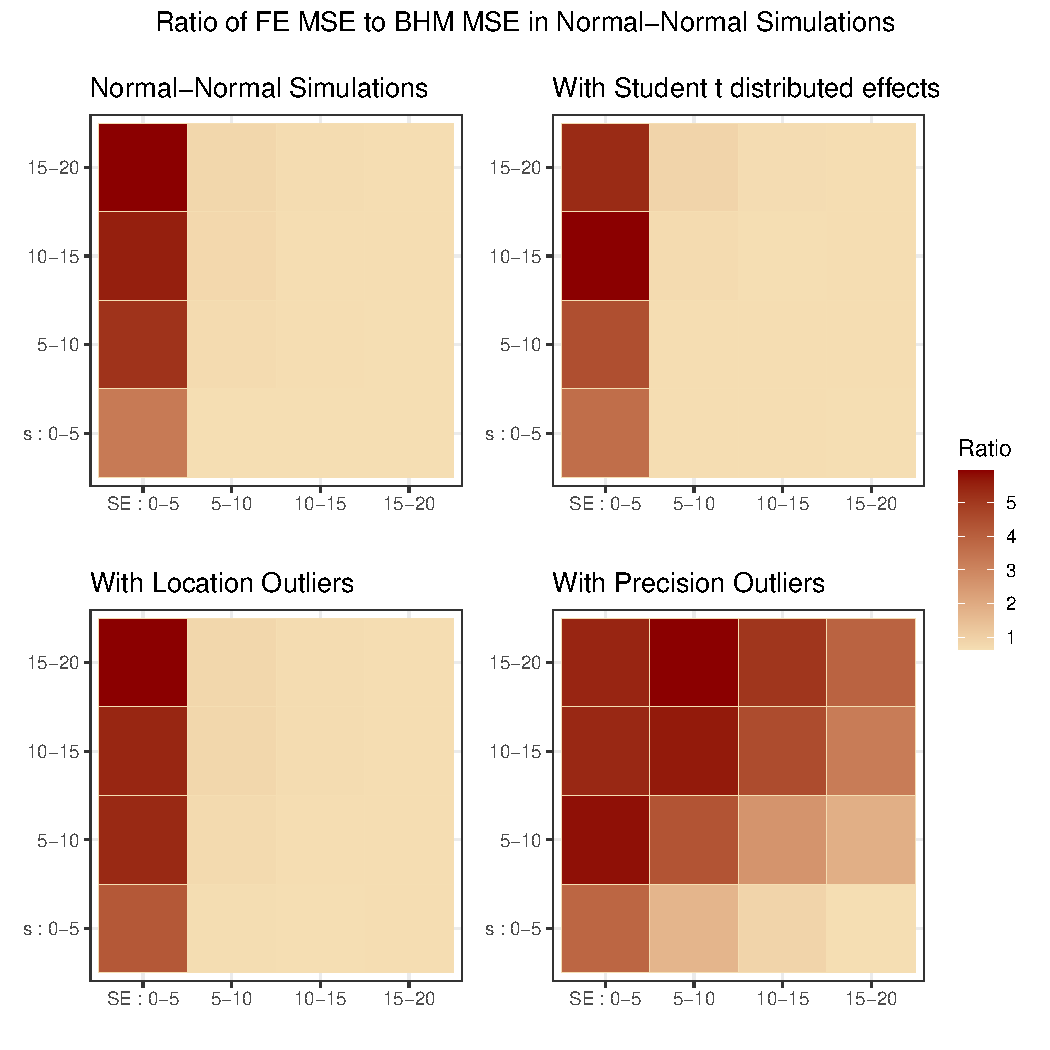
\includegraphics[scale=0.8]{heatmap_plots.pdf}
\caption{Heat maps showing value of (FE MSE)/(BHM MSE) for each simulation type}
\label{heatmaps}
\end{figure}

We now consider an alternative specification error in which the underlying data-generating process is a mixture distribution with potentially multiple modes. We first use a mixture distribution to create a classical outlier problem, which occurs when one site's true effect takes a value very different from the rest of the sites' true effects. However, in meta-analysis there is another potential type of outlier: one site may have a standard error that is very much smaller or larger than the rest of the sites' standard errors. We refer to this second type of outlier using the terminology ``precision outliers'', to distinguish from the more classical ``location outliers''. To my knowledge this paper constitutes the first attempt to formalize this problem, although meta-analytic issues created by differential precision have been noted in Higgins and Green (2011). We examine both types of outliers separately in the following simulations. 

Figure \ref{heatmaps}.3 shows the ratio of FE MSE to BHM MSE when the normal-normal DGP model has one site in which the true effect is generated by a normal that has been shifted away from the parent mean $\tau$. The results look quite similar to the normal-normal DGP results, with only slightly worse performance from the FE estimator in the upper left quadrant.

Figure \ref{heatmaps}.4 shows the ratio of FE MSE to BHM MSE when the normal-normal DGP model has one site in which the standard error is ten times smaller than the rest of the sites' standard errors on average. This makes a substantial difference in the relative performance of the FE estimator - it has double or triple the MSE of the BHM estimator in most of the grid area. In the worst case scenario for the FE it has MSE almost 6 times the size of the BHM estimator's MSE. In the worst case scenario for the BHM estimator, it still has roughly the same MSE as the FE estimator. Thus, in cases where one site is much more precise than all the others and there is no reason to believe effects are homogeneous, the BHM strongly outperforms the FE estimator.

Why does the fixed effects method perform so poorly in this case? While precision is unequivocally a good thing in a single study, it can be problematic in meta-analysis because precision and generalizability are two distinct but related properties. An estimate can be precise - and thus contain a lot of information about the site it comes from - without containing \emph{generalizable} information. In these simulations, the size of the effect which was much more precise was the same as the other effect sizes on average. All the site effects were a priori equally generalizable, and ex-post equally likely to be good indicators of the general effect $\tau$. But the highly precise effect was treated as more generalizable by the FE estimation process because this method has no way to distinguish precision and generalizability: indeed, if all effects are the same then precision actually is a perfect indicator of generalizability. 

By contrast, random effects methods can and must distinguish these two concepts because they must handle the possibility of heterogeneous effects. The BHM uses the concept of a parent distribution, and specifically the functional form of the parent distribution, to place each effect in context of the other effects. In the real world, the precision outlier is likely to be even more misleading for the FE estimator because that site's effect size is probably qualitatively different to the other sites. A study that is ten times more precise than all other studies may have a larger sample size because it is easier to collect data there, or it is more attractive to governments or NGOs to fund big studies there - these factors are probably correlated to the study's true effect size in some way. Thus, the relative reduction in MSE gained by using RE models in the presence of precision outliers is likely to be even greater than the results of these simulations suggest. 

\section{Vitamin A Supplements Reduce Child Mortality}

\subsection{Data}

In this section we repeat the meta-analysis of the impact of vitamin A supplementation on child mortality by using the same set of papers as the most recent study by Imdad et al (2022). Data are shown in Table~\ref{summary table}. 
As it is not easy to interpret a log standard error, we also display the upper and lower bounds of the confidence intervals implied by this log(se). 



In health literature, it is typical to model treatment effect on events data by using odds ratios (OR), risk ratios (RR), incidence risk ratios (IRR) or hazard ratios (HR). For example, in the vitamin A literature, including the meta-analysis models we cited, risk ratios between treatment and control groups are modeled. Since RR is approximately normal on logarithmic scale, we can apply the BHM from \eqref{rubin}. Data are shown in Table~\ref{summary table}. As it is not easy to interpret a log standard error, we also display the upper and lower bounds of the confidence intervals implied by this log(se).


Before proceeding, we note that an earlier meta-analysis by Mayo-Wilson et al. (2011) contains a very similar set of studies. Awasthi et al (2013) include only nine papers. We also repeated our analysis using the inputs from that paper to allow for direct comparison. The results for both RE and FE models are similar to Imdad et al. (2022) and we reach the same conclusions, therefore we do not show them here.


\subsection{Fixed-effects and random-effects models}

The previous theoretical analysis and simulation studies suggest that a random effects analysis using a Bayesian hierarchical model is typically a more appropriate choice of methodology for aggregating evidence relative to the FE model. While the FE estimator can beat the BHM when heterogeneity is small relative to sampling error, it rarely achieves a major reduction in MSE in the simulation study presented here. By contrast when the BHM beats the FE model it routinely achieves an MSE half as large, and in some cases can achieve an MSE less than 1/5th the size of its competitor's MSE. This is a very favourable efficiency versus robustness tradeoff, giving a strong argument to consider the RE model implemented via BHM as default choice for meta-analysis. 

The vitamin A literature is particularly suited to aggregation using RE because there is scientific and statistical evidence that underlying effects are heterogeneous across contexts and that this heterogeneity is likely large relative to the sampling error. 

Vitamin A studies we consider here differ in important ways, spanning several different countries, time periods, implementation and distribution methods and base rates of vitamin A deficiency in the populations studied. Supplementation only has theoretically-grounded medical benefits for individuals with a vitamin A deficiency. As a result, the rate of deficiency in the population is likely to have a major impact on the observed effect of supplementation on the population's risk ratio. 

There is also statistical evidence for heterogeneity, primarily that the 95\% confidence intervals for the risk ratios do not overlap in many of the studies. Both the DEVTA (2013) study's interval and the Herrera (1992) interval do not overlap with both the Rahmathullah (1990) interval and the Arthur (1992) interval. Indeed, the $\chi^2$ test results presented in Webtable 3 of Awasthi et al (2013) show strong evidence of heterogeneity: the authors do not discuss these results, but the low p-values in this context are indicative of heterogeneity (Cochrane Handbook Section 9.5.2). Moreover, the DEVTA study (Awasthi et al 2013) is almost an order of magnitude more precise than the other studies in the literature. This study is a precision outlier, and as we saw in the simulations, it is preferable to use an RE model in such a case.

All of the above suggests that BHM is appropriate methodology to aggregate the evidence on the effect of Vitamin A supplements on all-cause child mortality. We therefore fit both FE and RE models using Bayesian inference, which in turns allows us to compare them in terms of expected log predictive density.

%WW: cut this and move to Mayo-Wilson

%\subsection{Bayesian Hierarchical Analysis}


%The treatment effect in this literature is measured by a risk ratio that only takes positive values, so the Rubin (1981) model is not directly applicable to this case, but in the following sections we develop and apply an appropriate analogue.

%For the vitamin A literature, the empirical relative risk (RR) is the key object reported and used in the meta analyses in Imdad et al (2011) and Awasthi et al (2013). The relative risk statistic is defined:

%\begin{equation}
%\begin{aligned}
%\widehat{RR} = \frac{\text{Empirical probability of event in treatment group}}{\text{Empirical probability of event in control group}}.
%\end{aligned}
%\end{equation}

%This object only takes values on $R^+$ and thus cannot be modeled as normally distributed, but can be modeled as lognormally distributed around the true relative risk statistic with some sampling variation. Indeed, working with the RR on the log scale is considered the most suitable methodology in medical statistics according to Altman et al (1986) and  Gardner and Altman (1986, p750). Thus, Awasthi et al (2013) transform everything to the log scale to perform their meta-analysis, as shown in Webtable 3 of the supplementary appendix. In keeping with this approach, we use the following likelihood model for the Bayesian hierarchical meta-analysis:
%\begin{equation} \label{lognormal model}
%\begin{aligned}
%\widehat{RR}_k \sim \text{lognormal}(log(RR_k) , \widehat{logSE}_k) \; \forall \; k \\
%RR_k \sim  \text{lognormal}( log(RR), \sigma^2_{log(RR)}) \; \forall \; k .
%\end{aligned}
%\end{equation} 

%JM: does the following statement need more justification, or is this a common starting point in the literature?
For the BHM we use weakly informative priors centered at zero (no impact of the intervention):

\begin{equation} \label{lognormal priors}
\begin{aligned}
\log{RR} &\sim  \mathcal{N}(0,10^2) \\
\sigma^2_{\log{RR}} &\sim U[0,10].
\end{aligned}
\end{equation}



\subsection{ Results  }

%We fit the model described in equations \ref{lognormal model} with the standard diffuse but proper priors centered at the null of no impact as in equations \ref{lognormal priors}. The result is that the 

The results for Bayesian models with fixed and random effects are reported in Tables \ref{baggr-models-tab} (log scale) and \ref{baggr-tab-exp} (raw scale) and Figure \ref{baggr-density}. For the BHM of all studies we find the mean RR is 0.75 (95\% interval from 0.60 to 0.89), compared to 0.88 under FE model (95\% interval from 0.83 to 0.93). Our FE result is identical to the value reported by Imdad et al (2022), whereas for RE we find a marginally higher benefits than the original meta-analysis.\footnote{The difference is likely due to using BHM which, as mentioned in the Methodologies section, estimates higher heterogeneity than typical frequentist implementations of RE models in statistical software.}
The effect under RE model is more diffuse than under the FE model, but both models suggest that in the analysed sample of studies vitamin A supplements have on average considerably reduced child mortality. As we discussed in detail, the FE method gives a higher and more precise estimate of $RR$ because it does not take into account the heterogeneity across sites. 
%The BHM detects this heterogeneity and incorporates this into the dispersion of the posterior distribution of $\tau$. The resultingly wider 95\% interval shows that we should be much less confident in our specific point estimate of the general RR than the FE method suggests. 

Examining the posteriors for individual studies (Figure \ref{baggr-re}) shows that the effects are heterogeneous. This can also be seen based on summary statistics for the model: the average pooling factor is 0.34, suggesting that 66\% of the observed variation in estimated treatment effects is due to genuine differences between effects across studies (this value is typically referred to as $I^2$). However, heterogeneity is not precisely estimated, something that is typical to many meta-analyses of that size: Bayesian posterior 95\% interval for $I^2$ is (26\%, 91\%). This strongly suggests presence of some heterogeneity, but we cannot learn its extent based on the sample of 18 studies.

This heterogeneity is also reflected in the posterior predictive distribution of RR for the RE model. It has a mean of 0.78, with 95\% interval ranging from 0.4 to 1.3. (For the FE model it is by definition the same as the average effect.) This indicates that while we can be confident in the vitamin A effects within the analysed sample of studies, posterior predictive probability of RR being below 1 is 88\%.\footnote{We note that due to assumed normality of distribution of true effects the upper end of the distribution has a somewhat nonsensical interpretation: for example, the model implies a 2.5\% change of 30\% increase in the risk of mortality in a new study. Since we know that vitamin A supplementation is safe, a more appropriate model could consider a non-symmetrical distribution, with more probability mass concentrated around no effect rather than a harmful effect. Note, however, that this consideration is relevant for decision makers who are risk averse. In our case we focus on behaviour of the mean effect and do not consider the decision problem.}

Uncovering substantial heterogeneity prompts the question of why the impact is different across settings. In principle this question can be answered using contextual variables that describe differences in both the study designs and local contexts. In the vitamin A literature, there is presumably substantial variation in baseline vitamin A deficiency and the public health infrastructure that supports the intervention. The design of the trials also varies, particularly in the delivery mechanism which was direct in most cases but done via regional health centers in Awasthi et al (2013), leading to lower compliance with the supplement regime. Additionally, only some of the trials were double-blinded, and the intensity of the monitoring of outcomes per child differed dramatically across studies. 

Unfortunately, the original papers do not report sufficient information to permit the construction of quantitative variables suitable for statistical analysis. For example, many studies did not collect data on the control group rates of vitamin A deficiency, since observing cases of xerophthalmia and nightblindness in the children of the communities being studied is indicative of a severe enough deficiency to plausibly justify intervention. This rationale makes sense within each individual study, but has lead to a situation in which it is now impossible to determine how much heterogeneity is due to characteristics of studied populations versus study design. This serves as a reminder that collecting data on contextual variables in field trials is important for the scientific process. 


\subsection{Robustness to exclusion of DEVTA trial}

The debate over the design of the DEVTA trial and the resulting difference in compliance rates relative to other studies has lead some researchers to suggest that it should not be included in meta-analyses. Sommer, West and Martorell (2013) dispute Awasthi et al.'s (2013) claims about the effectiveness of the DEVTA trial's supplement delivery mechanism and patient compliance, finally commenting "At best, DEVTA is but one unorthodox study, done in one remote population of one country." 
%WW: The following is unclear. Why would you not include a program evaluation?
%JM: I have tried to clarify the language, but I think this point still needs to be addressed
They also note that DEVTA is properly a program evaluation. Given the disagreement about whether DEVTA really belongs with the other studies, it is debatable as to whether it should be included in the meta-analysis.

We report on the results of meta-analysis without the DEVTA trial in Table \ref{baggr-models-tab} and Figure \ref{baggr-density}. While the FE model is highly sensitive to exclusion of DEVTA, the RE model is much less affected. This difference between FE and RE models is illustrated in Figure 1, which shows strong overlap in p.p.d.'s for RE, but not FE, models.

It is important to also note that the heterogeneity estimate is not driven by exclusion of DEVTA. Whereas for 18 trials we found mean $I^2$ of 66\%, for the model of 17 trials we have $I^2 = 50\%$ (95\% interval from 1\% to 86\%). Thus the estimate of heterogeneity is even less precise, but on average the model still supports our concluson of heterogeneous effects.

Our result suggests that the DEVTA result does not substantially alter the evidence on typical effect of vitamin A supplements available from other studies and thus should not be taken as evidence that previous studies ``overestimated'' the effect in any major sense. Excluding the DEVTA trial also doesn't meaningfully change the estimated heterogeneity or pooling factors (Table \ref{baggr-models-tab}, columns 2 and 4).\footnote{This makes sense in the context of our simulations, since DEVTA is not a ``typical'' location outlier. Four other studies which we include in our analysis have found higher point estimates, associated with smaller positive effects and even negative effects on child mortality (Table \ref{summary table}, leftmost column).}

%Inclusion of DEVTA still has a small impact on the average effect in BHM because of substantial heterogeneity in the effects. Despite its high precision, the DEVTA estimate alone is not sufficient to overturn or outweigh the evidence in the previous cluster of results, which are symmetrically and quite widely dispersed around 0.75. 

%How heterogeneous are the effects across studies when DEVTA is excluded? The same pooling metric computed on the 8 remaining studies returns an average value of 0.31, indicating that substantial cross-study heterogeneity remains even without DEVTA. With DEVTA included, 71\% of the observed variation in estimated effects was attributed to genuine underlying heterogeneity; without DEVTA this number is 69\%, a minor reduction in heterogeneity. This makes sense because DEVTA is not a ``classical'' location outlier. Two other studies actually found higher point estimates, associated with smaller positive effects and even negative effects on child mortality, in the earlier literature (Vijayaraghavan et al 1990, Herrera 1992). 

%WW: how do we support the claim about the normal fitting well? Maybe later part of this paragraph is not necessary
%JM: this comment still needs actioning
Overall, the normal distribution of true effects seems to fit vitamin A studies we analysed very well and no single study appears pivotal to the result. The general pattern indicates that the typical effect should be somewhere in the region of RR=0.75, but the posterior predictive distribution of future impacts is not highly concentrated around this point, due to the heterogeneity.

The DEVTA result is a precision outlier, a type of result which, as we have shown in our simulations, may have a detrimental effect on the performance of the FE estimator in presence of heterogeneity. Precision outliers do not heavily impede the performance of BHMs because they are designed to detect heterogeneity and reweight the evidence accordingly. It is not the case that highly precise studies are ``underweighted'' or ``overweighted'' in any given method. Rather, when true treatment effect are heterogeneous any single estimate should not heavily influence the general estimate no matter how precise it is. While high precision indicates high information about the site $k$ in which the effect was estimated, this site is still just a singular data point in the set of $K$ data points. High precision does not necessarily indicate highly generalizable information. 


\subsection{Formal model selection using cross validation}

While our simulations and the high estimated heterogeneity are perhaps sufficient justification to choose an RE model over an FE alternative, we can also quantify the differences between the models by using a leave-one-out cross-validation approach (LOO CV).

For models without DEVTA trial, the performance of RE and FE models is very similar (RE elpd of -13.7, compared to FE elpd of -13.6).\footnote{In this case, i.e. when DEVTA trial is excluded, the choice between FE and RE models in this purely data-driven way is difficult. While the elpd value is not directly interpretable and 18 studies is not enough, both models are evenly matched in terms of number of studies for which they offer a better out-of-sample prediction (nine studies each).} However, when DEVTA trial is included, RE model still performs similarly (elpd of -14) while the FE model does not fit data anymore (elpd of -32.6). This can be best illustrated in Figure \ref{baggr-oos-ppc}, which once again visualises p.p.d.'s, but this time does so for 18 different models, each time leaving out one study and fitting meta-analysis model to the remaining 17. The impact of DEVTA trial is clearly visible, although we can see that there are also other studies for which the FE model is inadequate.

In summary, the LOO CV procedure justifies choice of an RE model regardless of whether the DEVTA trial is included in the set of meta-analysed studies.




\section{Conclusion}

The controversy in the vitamin A literature arose in part because of disagreements over the validity of using FE to aggregate the evidence, and the suitability of the RE alternative in this setting. Although Awasthi et al (2013) argued that RE models "conceal the reliability" of large trials and "give undue weight to small trials," the analysis presented in this paper shows that there are strong theoretical and empirical reasons to prefer the RE approach. While FE models are optimal under homogeneous treatment effects, RE models are optimal when the effects have underlying heterogeneity. When neither model describes the true data-generating structure, Monte Carlo simulation results show that the Bayesian hierarchical model either matches or outperforms the FE estimator by a wide margin in terms of MSE.

Using the same input data as the meta-analysis by Imdad et al (2022), a BHM estimates a typical reduction in the risk of child deaths of 26\%. 
We detected substantial heterogeneity in treatment effects, with 83\% of the observed variation attributed to genuine underlying differences across sites, although heterogeneity is not precisely estimated. The BHM results are robust to the inclusion or exclusion of the DEVTA study: despite its precision, it is only one study in a heterogeneous literature. Without DEVTA, the risk reduction is 29\%. 
Fundamentally, in the presence of heterogeneous treatment effects, precision in estimating average effect is not a sign of generalizability. 
Because the FE estimator cannot distinguish these two concepts, it underestimates the reduction in mortality risk, and is overly precise. 
This is in keeping with previous work showing the FE estimator typically overstates the precision of meta-analysis findings (Schmidt, Oh and Hayes, 2011) and thus the RE estimator is generally preferable when seeking to generalize beyond the set of studies in hand (Borenstein et al, 2010). 
%WW: How would you justify this next sentence?
%JM: I think this should either be removed or rephrased and put in the BHM subsection earlier in the paper
This analysis also confirms the advantages of the Bayesian approach to meta-analysis (Smith, Spiegelhalter, and Thomas, 1995).

The evidence shows that the general impact of vitamin A supplements on all-cause child mortality is substantial. However, it also suggests important differences in treatment effects across studies, and caution should be used before extrapolating from the studies in this literature into new settings. Given the biological mechanisms, vitamin A supplements should have a much larger effect on mortality when the population has a high rate of severe vitamin A deficiency, and this alone could account for the observed heterogeneity. However, study design could play an equally important role, given the major differences in delivery mechanism, compliance and monitoring across studies. Future work could explore the sources of this cross-site heterogeneity, and thus improve the effectiveness of the supplements in low-impact settings or target supplement programs more effectively to areas that need them most.

\clearpage

\begin{thebibliography}{99}

\bibitem{altman} Altman,  Douglas G. , David Machin, Trevor N. Bryant (1986), ``Statistics with confidence : confidence intervals and statistical guidelines'', BMJ Books, Bristol UK. 

\bibitem{arthur} Arthur, P., Kirkwood, B., Ross, D., Morris, S., Gyapong, J., Tomkins, A., \& Addy, H. (1992). ``Impact of vitamin A supplementation on childhood morbidity in northern Ghana''. \emph{The Lancet}, 339(8789), 361-362.

\bibitem{awasthi} Awasthi, S., Peto, R., Read, S., Clark, S., Pande, V., Bundy, D., \& the DEVTA (Deworming and Enhanced Vitamin A) team. (2013). ``Vitamin A supplementation every 6 months with retinol in 1 million pre-school children in north India: DEVTA, a cluster-randomised trial'' \emph{Lancet}, Vol 381.

\bibitem{BillMelinda} The Bill and Melinda Gates Foundation (2011) ``Nutritious Rice and Cassava Aim to Help Millions Fight Malnutrition'', Bill and Melinda Gates Foundation Press Release, accessed online at http://www.gatesfoundation.org/Media-Center/Press-Releases/2011/04/Nutritious-Rice-and-Cassava-Aim-to-Help-Millions-Fight-Malnutrition on March 15th 2016 

\bibitem{boren} Borenstein, M., Hedges, L. V., Higgins, J. P., \& Rothstein, H. R. (2010). "A basic introduction to fixed-effect and random-effects models for meta-analysis." Research synthesis methods, 1(2), 97-111.

\bibitem{brock} Brockwell, S. E., \& Gordon, I. R. (2001). "A comparison of statistical methods for meta-analysis". Statistics in medicine, 20(6), 825-840.

\bibitem{chung} Chung, Y., Rabe-Hesketh, S., Gelman, A., Liu, J., \& Dorie, V. (2012). ``Avoiding Boundary Estimates in Linear Mixed Models Through Weakly Informative Priors''. \emph{U.C. Berkeley Division of Biostatistics Working Paper Series}

\bibitem{cornell} Cornell JE, Mulrow CD, Localio R, Stack CB, Meibohm AR, Guallar E, et al. "Random-Effects Meta-analysis of Inconsistent Effects: A Time for Change". Ann Intern Med. ;160:267-270. doi: 10.7326/M13-2886

\bibitem{daualire} Daulaire, N. M., Starbuck, E. S., Houston, R. M., Church, M. S., Stukel, T. A., \& Pandey, M. R. (1992). ``Childhood mortality after a high dose of vitamin A in a high risk population''. \emph{BMJ}, 304(6821), 207-210.

\bibitem{field} Field, A. P. (2001). ``Meta-analysis of correlation coefficients: a Monte Carlo comparison of fixed-and random-effects methods''. \emph{Psychological methods}, 6(2), 161.

\bibitem{gardner} Gardner and Altman (1986) ``Confidence intervals rather than P values: estimation rather than hypothesis testing'' , \emph{British Medical Journal},Vol. 292.

\bibitem{garner} Garner, Paul, David Taylor-Robinson, and Harshpal Singh Sachdev (2013) ``DEVTA: results from the biggest clinical trial ever'' \emph{Lancet} Comment, Vol. 382.

\bibitem{gelmanpardoe} Gelman, Andrew, \& Iain Pardoe. ‘Bayesian Measures of Explained Variance and Pooling in Multilevel (Hierarchical) Models’. Technometrics 48, no. 2 (May 2006): 241–51. https://doi.org/10.1198/004017005000000517.

\bibitem{gelmanrubin} Gelman, A., \& Rubin, D. B. (1992)." Inference from iterative simulation using multiple sequences". Statistical science, 457-472.

\bibitem{gelman} Gelman, Andrew, Jessica Hwang, and Aki Vehtari. ``Understanding Predictive Information Criteria for Bayesian Models''. Statistics and Computing 24, no. 6 (November 2014): 997–1016. https://doi.org/10.1007/s11222-013-9416-2.

\bibitem{hedges} Hedges, L. V., \& Vevea, J. L. (1998). ``Fixed-and random-effects models in meta-analysis''. \emph{Psychological methods}, 3(4), 486.

\bibitem{herrera} Herrera, M. G., Nestel, P., Weld, L., El Amin, A., Mohamed, K. A., \& Fawzi, W. W. (1992). ``Vitamin A supplementation and child survival''. \emph{The Lancet}, 340(8814), 267-271.

\bibitem{cochrane} Higgins, J. P. and Sally Green (Eds) (2011) "Cochrane handbook for systematic reviews of interventions" (Version 5.1.0). Chichester: Wiley-Blackwell.

\bibitem{higgy} Higgins, J. P., \& Thompson, S. G. (2002). "Quantifying heterogeneity in a meta-analysis". Statistics in medicine, 21(11), 1539-1558.

\bibitem{imdad2011} Imdad et al (2011), ``Impact of Vitamin A supplementation on infant and childhood mortality'' \emph{BMC Public Health}, Vol. 11.

\bibitem{imdad2022} Imdad et al (2022), ``Vitamin A Supplementation for Preventing Morbidity and Mortality in Children from Six Months to Five Years of Age'' \emph{Cochrane Database of Systematic Reviews}, no. 3 (2022).

\bibitem{iwata} Iwata, M., Hirakiyama, A., Eshima, Y., Kagechika, H., Kato, C., \& Song, S. Y. (2004). ``Retinoic acid imprints gut-homing specificity on T cells''. \emph{Immunity}, 21(4), 527-538.

\bibitem{james} James, W. and C. Stein (1961) ``Estimation with Quadratic Loss'', \emph{Proc. Fourth Berkeley Symp. on Math. Statist. and Prob.}, Vol. 1 (Univ. of Calif. Press, 1961), 361-379

\bibitem{mora} Mora, J. R., Iwata, M., \& von Andrian, U. H. (2008). ``Vitamin effects on the immune system: vitamins A and D take centre stage''. \emph{Nature Reviews Immunology}, 8(9), 685-698.

\bibitem{overton} Overton, R. C. (1998). ''A comparison of fixed-effects and mixed (random-effects) models for meta-analysis tests of moderator variable effects''. \emph{Psychological methods}, 3(3), 354.

\bibitem{rahmathullah} Rahmathullah, L., Underwood, B. A., Thulasiraj, R. D., Milton, R. C., Ramaswamy, K., Rahmathullah, R., \& Babu, G. (1990). ``Reduced mortality among children in southern India receiving a small weekly dose of vitamin A''. \emph{New England journal of medicine}, 323(14), 929-935.

\bibitem{rubin81} Rubin, D. B. (1981). "Estimation in parallel randomized experiments. Journal of Educational and Behavioral Statistics", 6(4), 377-401.

\bibitem{schmidt} Schmidt, F. L., Oh, I. S., \& Hayes, T. L. (2009). "Fixed-versus random-effects models in meta-analysis: Model properties and an empirical comparison of differences in results". British Journal of Mathematical and Statistical Psychology, 62(1), 97-128.

\bibitem{smith} Smith, T. C., Spiegelhalter, D. J., \& Thomas, A. (1995). Bayesian approaches to random-effects meta-analysis: a comparative study. Statistics in medicine, 14(24), 2685-2699.

\bibitem{sommer13} Sommer, Alfred, Keith P West Jr, and Reynaldo Martorell (2013) ``Vitamin A Supplementation in Indian Children'', \emph{Lancet} Comment, Vol. 382.

\bibitem{sommer86} Sommer, A., Djunaedi, E., Loeden, A. A., Tarwotjo, I., West, K., Tilden, R., ... \& Aceh Study Group. (1986). ``Impact of vitamin A supplementation on childhood mortality: a randomised controlled community trial''. \emph{The Lancet}, 327(8491), 1169-1173.

\bibitem{sommer83} Sommer, A., Hussaini, G., Tarwotjo, I., \& Susanto, D. (1983). ``Increased mortality in children with mild vitamin A deficiency''. \emph{The Lancet}, 322(8350), 585-588.

\bibitem{turner} Turner, R. M., Jackson, D., Wei, Y., Thompson, S. G., \& Higgins, J. P. T. (2015). ``Predictive Distributions for Between-Study Heterogeneity and Simple Methods for Their Application in Bayesian Meta-Analysis''. \emph{Statistics in Medicine} 34, no. 6 : 984–98.

\bibitem{unicef} United Nations Childrens Fund (UNICEF) (2007) ``Vitamin A Supplementation: A Decade Of Progress'' , UNICEF Report. 

\bibitem{VAST} Ross, D. A., Dollimore, N., Smith, P. G., Kirkwood, B. R., Arthur, P., Morris, S. S., ... \& Ghana VAST Study Team. (1993). ``Vitamin A supplementation in northern Ghana: effects on clinic attendances, hospital admissions, and child mortality''. \emph{The Lancet}, 342(8862), 7-12.

\bibitem{vij} Vijayaraghavan, K., Radhaiah, G., Prakasam, B. S., Sarma, K. R., \& Reddy, V. (1990). ``Effect of massive dose vitamin A on morbidity and mortality in Indian children''. \emph{The Lancet}, 336(8727), 1342-1345.

\bibitem{wasserstein} Wasserstein, R. L., \& Lazar, N. A. (2016).''The ASA's statement on p-values: context, process, and purpose''. \emph{The American Statistician}, (just-accepted), 00-00.

\bibitem{west} West, K. P., Katz, J., LeClerq, S. C., Pradhan, E. K., Tielsch, J. M., Sommer, A., ... \& Pandey, M. R. (1991). ``Efficacy of vitamin A in reducing preschool child mortality in Nepal''. \emph{The Lancet}, 338(8759), 67-71.

\bibitem{WHO} World Health Organisation (2016) ``Nutrition: Micronutrient Deficiencies: Vitamin A'', accessed online at http://www.who.int/nutrition/topics/vad/en/ on March 15th 2016


\end{thebibliography}


% \begin{figure}[ht]
% \includegraphics[scale=0.8]{vitamin_a_data_summary.pdf}
% \caption{All input data for the meta-analysis of Awasthi et al (2013).}
% \label{summary table}
% \end{figure}

\begin{table}
\label{summary table}
\caption{Input data and study-level results for BHM based on studies included in Imdad et al (2022). RR is mean risk ratio. LCI and UCI are lower and upper ends of the 95\% intervals. SE refers to standard error of the log(RR).}
\begin{tabular}[t]{lrrrrrrrr}
\toprule
\multicolumn{1}{c}{} & \multicolumn{5}{c}{Observed (risk ratio)} & \multicolumn{3}{c}{Posterior (risk ratio)} \\
\cmidrule(l{3pt}r{3pt}){2-6} \cmidrule(l{3pt}r{3pt}){7-9}
Study & RR & LCI & UCI & log(RR) & SE & RR & LCI & UCI\\
\midrule
Agarwal 1995 & 1.22 & 0.66 & 2.25 & 0.20 & 0.31 & 0.90 & 0.62 & 1.41\\
Barreto 1994 & 1.00 & 0.14 & 7.08 & 0.00 & 1.00 & 0.76 & 0.42 & 1.31\\
Benn 1997 & 0.46 & 0.14 & 1.47 & -0.78 & 0.59 & 0.70 & 0.38 & 1.10\\
Chowdhury 2002 & 0.14 & 0.03 & 0.63 & -1.94 & 0.75 & 0.63 & 0.30 & 1.00\\
Daulaire 1992 & 0.74 & 0.55 & 0.99 & -0.30 & 0.15 & 0.75 & 0.58 & 0.95\\
\addlinespace
DEVTA 2013 & 0.96 & 0.89 & 1.03 & -0.04 & 0.04 & 0.95 & 0.88 & 1.02\\
Dibley 1996 & 0.33 & 0.01 & 7.98 & -1.12 & 1.63 & 0.73 & 0.38 & 1.24\\
Donnen 1998 & 0.60 & 0.23 & 1.55 & -0.51 & 0.48 & 0.72 & 0.43 & 1.12\\
Fisker 2014 & 0.93 & 0.66 & 1.31 & -0.07 & 0.17 & 0.86 & 0.66 & 1.15\\
Herrera 1992 & 1.06 & 0.82 & 1.37 & 0.06 & 0.13 & 0.97 & 0.77 & 1.24\\
\addlinespace
Pant 1996 & 0.57 & 0.37 & 0.88 & -0.56 & 0.22 & 0.66 & 0.45 & 0.90\\
Rahmathullah 1990 & 0.46 & 0.30 & 0.71 & -0.78 & 0.22 & 0.59 & 0.39 & 0.83\\
Ross 1993 (health) & 0.30 & 0.12 & 0.74 & -1.22 & 0.47 & 0.61 & 0.32 & 0.95\\
Ross 1993 (survival) & 0.81 & 0.67 & 0.97 & -0.21 & 0.09 & 0.80 & 0.68 & 0.95\\
Sommer 1986 & 0.73 & 0.54 & 1.00 & -0.31 & 0.15 & 0.74 & 0.58 & 0.96\\
\addlinespace
Venkatrao 1996 & 0.37 & 0.10 & 1.37 & -1.00 & 0.67 & 0.68 & 0.36 & 1.09\\
Vijayaraghavan 1990 & 1.02 & 0.57 & 1.82 & 0.02 & 0.30 & 0.85 & 0.59 & 1.27\\
West 1991 & 0.70 & 0.56 & 0.88 & -0.36 & 0.12 & 0.71 & 0.58 & 0.87\\
\bottomrule
\end{tabular}
\end{table}

\begin{table}
\caption{Comparison of results of all four meta-analysis models fitted to our data, on log(RR) scale.}
\label{baggr-models-tab}
\centering
\resizebox{\linewidth}{!}{
\begin{tabular}[t]{lllll}
\toprule
  & Hypermean & Hyper-SD & p.p.d. & Pooling\\
\midrule
\textbf{Partial, all data} & \textbf{-0.29 (-0.51, -0.12)} & \textbf{0.25 (0.094, 0.51)} & \textbf{-0.29 (-0.93, 0.27)} & \textbf{0.66 (0.26, 0.91)}\\
Partial, no DEVTA & -0.32 (-0.53, -0.15) & 0.23 (0.025, 0.51) & -0.32 (-0.92, 0.22) & 0.5 (0.015, 0.86)\\
Full, all data & -0.13 (-0.18, -0.068) & 0 (0, 0) & -0.13 (-0.18, -0.068) & 1 (1, 1)\\
Full, no DEVTA & -0.26 (-0.36, -0.17) & 0 (0, 0) & -0.26 (-0.36, -0.17) & 1 (1, 1)\\
\bottomrule
\end{tabular}}
\end{table}

\begin{table}
\caption{Comparison of results on the risk ratio (non-log) scale.}
\label{baggr-tab-exp}
\begin{tabular}[t]{lrr}
\toprule
Pooling model & Hypermean & p.p.d.\\
\midrule
\textbf{Partial, all data} & \textbf{0.75 (0.60, 0.89)} & \textbf{0.78 (0.40, 1.30)}\\
Partial, no DEVTA & 0.73 (0.58, 0.86) & 0.76 (0.40, 1.30)\\
Full, all data & 0.88 (0.83, 0.93) & 0.88 (0.83, 0.93)\\
Full, no DEVTA & 0.77 (0.70, 0.84) & 0.77 (0.70, 0.84)\\
\bottomrule
\end{tabular}
\end{table}

\begin{figure}[h!]
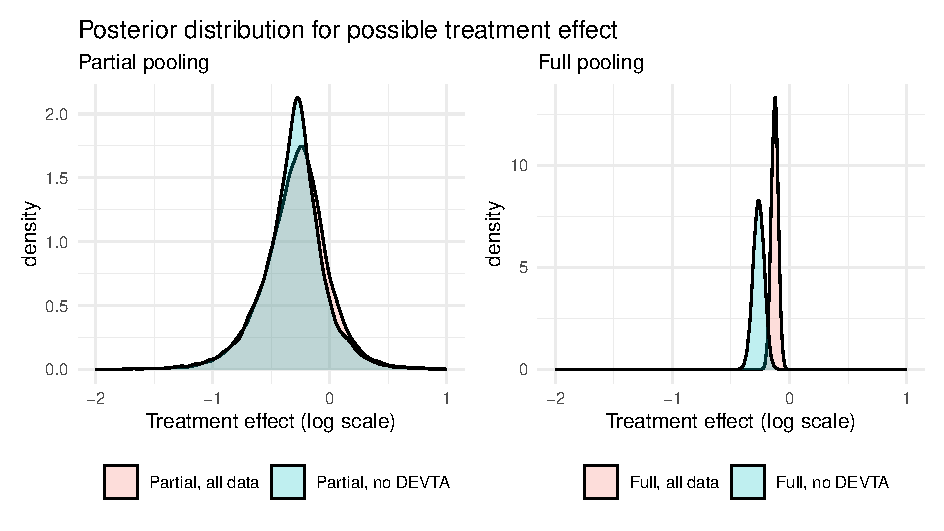
\includegraphics{baggr-density.pdf}
\caption{Illustration of how marginal posterior of meta-analytic risk ratio changes with inclusion/exclusion of DEVTA trial, for random-effects models (left panel) and for fixed-effects models (right panel)}
\label{baggr-density}
\end{figure}

\begin{figure}[h!]
\centering
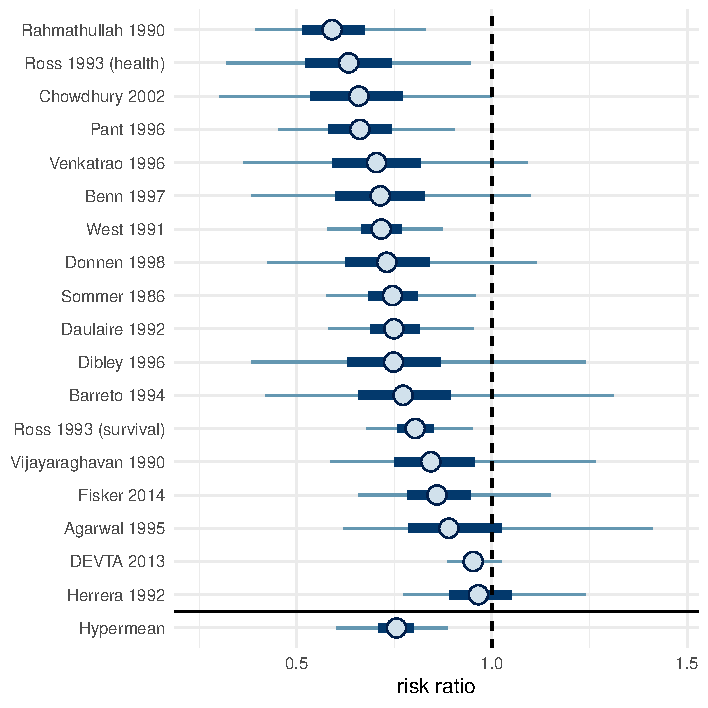
\includegraphics{baggr-re.pdf}
\caption{Marginal posteriors for the 9 RR values and originally reported RR statistics} \label{baggr-re}
\end{figure}

\begin{figure}[h!]
\centering
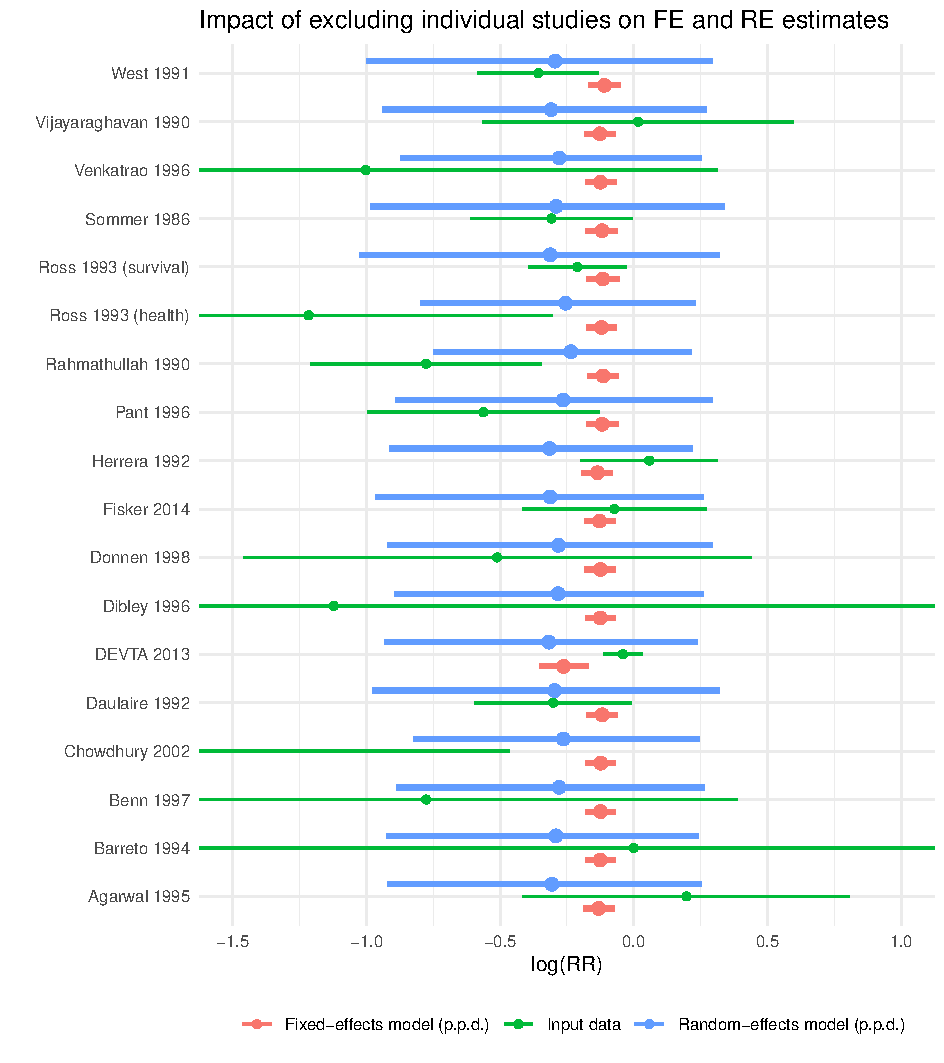
\includegraphics{baggr-oos-ppc.pdf}
\caption{Posterior predictive distributions (in blue and red) compared to treatment effect estimates reported in each study (green). Each row shows fixed-effects (red) and random-effects (red) models fit to data where we exclude that particular study. The interval represents posterior predictive distribution, which can be thought of as the distribution of effects for an unobserved study. Note how in some cases the FE p.p.d. does not overlap with studies; in particular for the DEVTA study. Note that the estimates for FE model change when we exclude DEVTA trial, but this does not occur for the RE model.} \label{baggr-oos-ppc}
\end{figure}

\end{document}
